\section{Archive Process Implementation}
This section gives an overview of the architecture of the archive process that is responsible
for moving the project data to the Synology. 

The archive process is a complex 
task, thus involves many operations and communications. Figure \ref{fig:archiveClassDiagram} illustrates the class diagram for the archive process. This diagram depicts only the top level classes
which perform actions (e.g., archiving files, archiving simulation result). The operations include HTTP GET request to an external service, storing of received
data into the Synology, and forwarding the received data to the next component which requires it. This involves a large number of classes and cannot be 
illustrated in a single diagram. This diagram is shown to point out the order of complexity that the archive process undergoes and the way in which it is
implemented. Also, to make the modules of the archive service more reusable the components are separated into several classes
like ArchiveMetadata, ArchiveScenarios etc. This separation
of classes later allows an easier extension. It could be the case that in future a new requirement
that involves the Archive service to only archive
the input files arises. In this case, as the components are already separated, one can use the interface of ArchiveFile for a quick implementation. 
Besides, different design patterns have been used
in the Archive service like the Repository pattern \cite{repo} to help make the software more coherent.
 
\subsubsection{Repository Pattern Implementation}
Many components require access to the Synology storage to archive their respective data, that presents a problem of having data
persistence logic duplication in many components. To solve this, the repository pattern will be implemented where there would be an abstraction layer, i.e., a repository
provides the query interface to the component. This abstraction layer is injected to the required components and they can call the 
method to carry out persistence actions (CRUD). Also, this also decouples the component from the type of storage being used ,i.e., Synology, so it does not
matter for the component if the type of storage is changed from Synology to something else since it just needs the interface for persistence. Figure 
\ref{fig:repositoryPattern} illustrates how the repository acts as an abstraction layer for the client aiding the system to be more cohesive. 
\begin{figure}[H]
    \centering 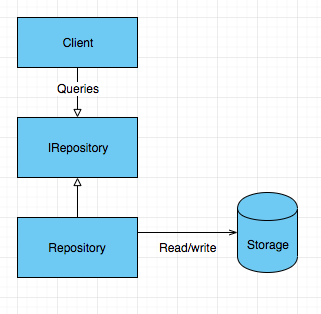
\includegraphics[scale=0.7]{grafiken/repositoryPattern.png}
    \caption{Repository Pattern overview}
    \label{fig:repositoryPattern}
\end{figure}


\begin{figure}[H]
    \centering 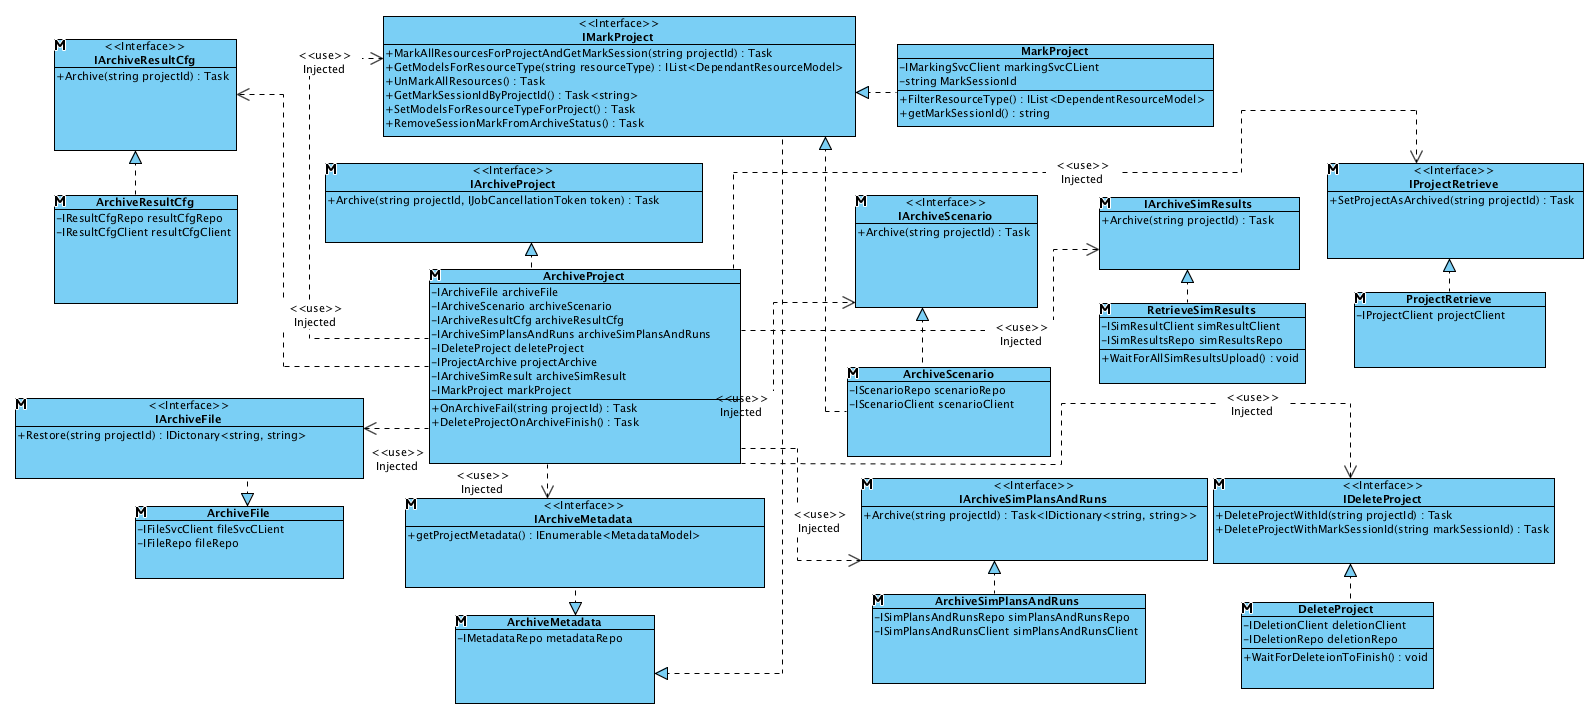
\includegraphics[height=6.5cm, angle=90, origin=c, width=11cm]{grafiken/archiveClass.png}
    \caption{Class Diagram for the Archive process (Top level)}
    \label{fig:archiveClassDiagram}
\end{figure}
